\documentclass[%
 reprint,
 superscriptaddress,
 amsmath,amssymb,
 aps,
 pre,
 floatfix,
]{revtex4-2}

% --- Encoding and language ---
\usepackage[utf8]{inputenc}
\usepackage[T1]{fontenc}
\usepackage[english]{babel}
\usepackage{microtype}
\usepackage{xspace}
\usepackage{xcolor}

% --- Mathematics and symbols ---
\usepackage{mathrsfs, stmaryrd}
\usepackage{siunitx}
\usepackage{bm}

% --- Graphics and figures ---
\usepackage{graphicx}
\usepackage{subcaption}   % si problème avec revtex, utiliser \usepackage{subfig}
\graphicspath{{pictures/}}
\usepackage{placeins}   % pour \FloatBarrier

% --- Tables ---
\usepackage{booktabs}
\usepackage{multirow, array, makecell}
\usepackage{dcolumn}

% --- Lists ---
\usepackage{enumitem}

% --- Algorithms and code ---
\usepackage[ruled,vlined]{algorithm2e}
\usepackage{listings}
\usepackage{fvextra}
\usepackage{tikz}
\usetikzlibrary{decorations.pathreplacing}

% --- References (hyperref avant cleveref) ---
\usepackage{hyperref}
\usepackage{cleveref}
\crefname{algocf}{algorithm}{algorithms}
\Crefname{algocf}{Algorithm}{Algorithms}

% --- Macros : annotations (à retirer avant soumission) ---
\newcommand{\noteBastien}[1]{\textcolor{blue}{#1}}
\newcommand{\noteMichele}[1]{\textcolor{red}{#1}}
\newcommand{\noteDavid}[1]{\textcolor{green}{#1}}

% --- Macros : code identifiers ---
\newcommand{\UnsignedInt}{\texttt{UnsignedInt}\xspace}
\newcommand{\UnsignedInts}{\texttt{UnsignedInts}\xspace}
\newcommand{\BitSet}{\texttt{BitSet}\xspace}
\newcommand{\BitSets}{\texttt{BitSets}\xspace}
\newcommand{\Bits}{\texttt{Bits}\xspace}

\begin{document}

\title{Dynamical properties of the Hopfield model\\through bitwise arithmetic}

\author{Bastien Dumont}
 \affiliation{Aix-Marseille Universit\'e, Marseille, France}
 \affiliation{Universit\'e Paris-Saclay, Orsay, France}

\author{David Lacoste}
 \affiliation{Gulliver Laboratory, CNRS UMR 7083, ESPCI Paris, PSL Research University, Paris, France}

\author{Michele Castellana}
 \affiliation{Institut Curie, PSL Research University, CNRS UMR 168, Paris, France}

\date{\today}

\begin{abstract}
The Hopfield model, introduced in its now-canonical form by J.J. Hopfield in 1982, laid the foundation for the understanding of neural networks, whether they are biological or artificial. This model has become a reference in the statistical mechanics of networks and its equilibrium properties have been extensively studied and are now well understood. Nevertheless, much remains to be discovered about the dynamics leading to those equilibrium properties. Studying such dynamical properties requires the use of optimized algorithms capable of probing large samples of trajectories or initial conditions, as well as potentially rare events. In this internship project, we use a bitwise implementation of the Metropolis algorithm to study the properties of several discrete-value network models such as the Ising model, the Edwards-Anderson model and the Hopfield model. This implementation takes advantage of the native machine-specific binary arithmetic to efficiently simulate the evolution of $n_\text{bits}$ systems in parallel. We show that this approach is well-adapted to simulate discrete value models, and in particular the Hopfield network, and can also yield significant computational gains when properly implemented at the low level.
\end{abstract}
%\keywords{Suggested keywords}%Use showkeys class option if keyword
                              %display desired
\maketitle

%\tableofcontents
\section{Introduction}


\subsection{Subject}
 In October 2024, John J. Hopfield was awarded the Nobel Prize in Physics alongside Geoffrey Hinton for their
pioneering work on artificial neural networks \cite{nobel2024physics}. Their work laid the foundations for further development and understanding of neural networks, whether they are organic or artificial, and eventually gave rise to Artificial Intelligence (AI).\\
Hopfield worked on an artificial neural network originally invented by Shun'ichi Amari in 1972 \cite{Amari1972LearningPA}. He greatly contributed to the analysis, understanding and popularization of the network in his landmark paper \textit{Neural networks and physical systems with emergent collective computational abilities} published in 1982 \cite{Hopfield1982}, and the network was eventually named after him. The model, described in more details in subsection \ref{subsec:hopfield_model}, is similar to the Ising and the spin glass networks: it is composed of a set of spins -- called neurons in the case of the Hopfield network -- $S_i \in \{-1, 1\}$ interacting with one another. In the same way as the two preceding models, the Hopfield model is energy-based, that is it will tend to minimize its energy over time. What makes this model different from the other two is the way the interactions between neurons are defined: as for the Ising and spin glass models they remain static over time but depend on the set of patterns to be stored in the network, making the latter attractors, that is to say minima of energy, of the dynamics. \\
The Hopfield model provided the first simple yet powerful framework for understanding networks of interconnected neurons. It has become a reference in statistical mechanics on networks and its properties at equilibrium have been extensively studied and are now well known, whether it is its statistical mechanics \cite{Amit1985,AMIT1987,Amit1989,Sompolinsky1988} or its phase diagram and transitions \cite{Hertz1991}. However, much less is known about the dynamics that lead to those well-known equilibrium properties.

\subsection{Objectives}
The main objective of this internship is to efficiently simulate the Metropolis dynamics on the Hopfield network. To this end, we use a bitwise formalism that allows us to simulate several replicas of the system in parallel, increasing the efficiency of the exploration of the model's energy landscape. Our objectives in this internship are thus twofold: first, to validate the bitwise implementation and quantify its computational gain in yield over the standard Metropolis algorithm;
second, to leverage this implementation to study the dynamics of the Hopfield network. To validate the implementation, we begin with the Ising model, which serves as a natural benchmark due to its simplicity and well-characterized phase transition. Once this implementation has been proven sane and efficient on the Ising network, we increase the complexity by implementing it on the spin glass network, testing the gain in yield again.\\
Once the bitwise arithmetic has been validated on both models, we implement it on the Hopfield network in order to analyze its dynamics.


\section{Implementation of the algorithm}
We start by presenting the broad implementation of the Metropolis algorithm, before showing how we adapt it to each specific model.
\subsection{The Metropolis algorithm}
In order to make the models evolve in time, which is necessary to observe their dynamics, we use the well-known metropolis algorithm \cite{Metropolis1953}. For models with a defined Hamiltonian, the Metropolis algorithm proceeds as follows:
\begin{enumerate}
    \item Start from an initial configuration $\{S_i\}$.
    \item Repeat $N$ times:
    \begin{enumerate}[label=\alph*.]
        \item Pick a random spin $S_k$ and compute the energy change $\Delta E_k$
              upon flipping it.
        \item If $\Delta E_k \leq 0$, accept the flip.
        \item Else, draw a random number $r \sim \mathcal{U}([0,1])$
              and accept the flip if $r \leq e^{-\beta \Delta E_k}$.
    \end{enumerate}
    \item Repeat Step 2 for $N_{\text{sweeps}}$ sweeps.
\end{enumerate}
Where $N$ is the number of spins, $\beta$ is the inverse temperature,
and $N_{\text{sweeps}}$ is the number of sweeps, where one sweep consists of
$N$ successive single-spin flip attempts.\\
This algorithm however becomes computationally demanding when one attempts to sample a large number of configurations. This situation occurs, for example, when looking for rare samples in the dynamics, or sampling many different initial conditions -- both of which we will try to explore during this internship. We thus need to find way of optimizing the implementation of the algorithm.

\subsection{First optimization: the bitwise arithmetic}
The first optimization in the implementation of the Metropolis algorithm is the use of bitwise arithmetic. The main idea is to leverage the boolean representation as stored in our computers. The typical object that we manipulate is called \Bits: it is a collection of $n_\text{bits}=64$ boolean variables. In that way, we have the possibility to simulate $64$ evolutions of the same variable in parallel.
\begin{figure}[ht]
\centering
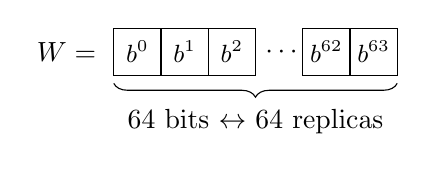
\begin{tikzpicture}

\def\boxw{0.6} % largeur exacte de la boîte
\def\step{\boxw} % PAS = largeur => boîtes collées

% left boxes
\foreach \i/\label in {0/0, 1/1, 2/2} {
    \draw (\i*\step, 0) rectangle (\i*\step+\boxw, 0.6);
    \node[font=\small] at (\i*\step+0.3, 0.3) {$b^{\label}$};
}
% ...
\node at (3*\step+0.33, 0.3) {$\cdots$};

% right boxes
\foreach \i/\label in {0/62, 1/63} {
    \draw (4*\step + \i*\step, 0)
        rectangle (4*\step + \i*\step+\boxw, 0.6);
    \node[font=\small] at (4*\step + \i*\step+0.3, 0.3)
        {$b^{\label}$};
}

% left label
\node at (-0.6, 0.3) {$W=$};

% Brace below
\draw[decorate, decoration={brace, amplitude=5pt, mirror}]
    (0, -0.1) --
    (6*\step, -0.1)
    node[midway, below=6pt] {64 bits $\leftrightarrow$ 64 replicas};

\end{tikzpicture}
\caption{A \Bits $W$ encoding 64 parallel replicas. Each bit $b^k$ carries the state of replica $k$.}
\label{fig:Bits}
\end{figure}

This structure is very convenient to represent binary variable such as the spins of the system. The boolean representation $b^k \in \{0,1\}$ of a spin $s^k \in \{-1,+1\}$ is given by $b^k = (s^k+1)/2$. In that way, we are able to implement several replicas of the full spin system in a set of \Bits $\{S_i\}$, each encoding the replicas of the associated spin, as shown in Figure~\ref{fig:spins_Bits}.

\begin{figure}[t]
\centering
\def\svgwidth{0.28\linewidth}
\input{pictures/spins_Bits.pdf_tex}
\caption{Bitwise implementation of a spin system. Each replica of the entire system is obtained by selecting the corresponding replica in each spin.}
\label{fig:spins_Bits}
\end{figure}
Storing all replicas in a single \Bits object allows us to manipulate and update them simultaneously using a single bitwise operator. This is an instance of SWAR (SIMD Within A Register) parallelism, where SIMD stands for Single Instruction, Multiple Data: all 64 replicas are updated by a single bitwise instruction. The restriction to $n_\text{bits} = 64$ reflects the native word size of modern 64-bit CPUs \cite{intel2023sdm}. This could in principle be extended to 512 bits using AVX-512 SIMD instructions, at the cost of introducing a new register type in the implementation.\\
The convention used for what follows is presented in the Table \ref{tab:notation}:
\begin{table}[h]
\centering
\begin{tabular}{ll}
\hline
Object & Notation \\
\hline

$n_\text{bits}$ replicas of spin i & $S_i \in \{-1,1\}^{n_\text{bits}}$ \\
$n_\text{bits}$-bit word (\Bits) & $B_i \in \{0,1\}^{n_\text{bits}}$ \\
Replica $k$ of spin $i$ & $s_i^{(k)} \in \{-1,+1\}$ \\
Replica $k$ of bit $i$ & $b_i^{(k)} \in \{0,1\}$ \\
\hline
\end{tabular}
\caption{Notation for the bitwise representation of spins.}
\label{tab:notation}
\end{table}

Now that we know how to conveniently handle binary variables such as spins, we need to employ the same formalism to represent integer, such as the sum $\Delta E_k$. This is done using a \BitSet, which is a collection of \Bits. When each \Bits is associated with a power of 2, the \BitSet represent a collection of $n_\text{bits}$ unsigned integers and the \BitSet is called \UnsignedInt. We show an example of \UnsignedInt in the Figure~\ref{fig:UnsignedInt}.

\begin{figure}[ht]
\centering
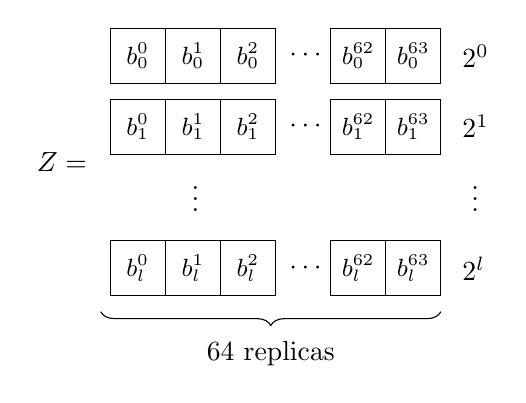
\begin{tikzpicture}

\def\boxsize{0.7}
\def\gap{0.12} % <-- horizontal spacing
\def\step{\boxsize+\gap}
\def\rowsep{0.9}

\tikzset{
    bitbox/.style={
        draw,
        minimum size=\boxsize cm,
        inner sep=0pt,
        font=\small,
        align=center
    }
}

% Left label
\node[left] at ({-0.05},{-1.5*\rowsep+0.5*\boxsize}) {$Z=$};

% Row k=0
\foreach \i/\clabel in {0/0,1/1,2/2}{
    \node[bitbox] at ({\i*\step+0.5*\boxsize},{0.5*\boxsize})
        {$b_{0}^{\clabel}$};
}

\node at ({3*\step+0.38},{0.5*\boxsize}) {$\cdots$};

\foreach \i/\clabel in {0/62,1/63}{
    \node[bitbox] at ({(4+\i)*\step+0.5*\boxsize},{0.5*\boxsize})
        {$b_{0}^{\clabel}$};
}

\node[right] at ({6*\step+0.15},{0.5*\boxsize}) {$2^0$};

% Row k=1
\foreach \i/\clabel in {0/0,1/1,2/2}{
    \node[bitbox] at ({\i*\step+0.5*\boxsize},{-\rowsep+0.5*\boxsize})
        {$b_{1}^{\clabel}$};
}

\node at ({3*\step+0.38},{-\rowsep+0.5*\boxsize}) {$\cdots$};

\foreach \i/\clabel in {0/62,1/63}{
    \node[bitbox] at ({(4+\i)*\step+0.5*\boxsize},{-\rowsep+0.5*\boxsize})
        {$b_{1}^{\clabel}$};
}

\node[right] at ({6*\step+0.15},{-\rowsep+0.5*\boxsize}) {$2^1$};

% Dots
\node at ({1.55*\step},{-1.9*\rowsep+0.5*\boxsize}) {$\vdots$};
\node at ({6.05*\step+0.4},{-1.9*\rowsep+0.5*\boxsize}) {$\vdots$};

% Row k=l
\foreach \i/\clabel in {0/0,1/1,2/2}{
    \node[bitbox] at ({\i*\step+0.5*\boxsize},{-3*\rowsep+0.5*\boxsize})
        {$b_{l}^{\clabel}$};
}

\node at ({3*\step+0.38},{-3*\rowsep+0.5*\boxsize}) {$\cdots$};

\foreach \i/\clabel in {0/62,1/63}{
    \node[bitbox] at ({(4+\i)*\step+0.5*\boxsize},{-3*\rowsep+0.5*\boxsize})
        {$b_{l}^{ \clabel}$};
}

\node[right] at ({6*\step+0.15},{-3*\rowsep+0.5*\boxsize}) {$2^{l}$};

% Bottom brace
\draw[
    decorate,
    decoration={brace,amplitude=5pt,mirror}
]
({0},{-3*\rowsep-0.2})
--
({6*\step},{-3*\rowsep-0.2})
node[midway,below=7pt] {64 replicas};
\end{tikzpicture}
\caption{An \UnsignedInt encoding 64 parallel unsigned integers. Each row is a \Bits associated with a power of 2. The value of each integer is obtained by reading the \UnsignedInt along the corresponding column. For instance, the fifth integer stored in $Z$ is $Z_4=\sum\limits_{i=0}^l b_i^4\, 2^i$.}
\label{fig:UnsignedInt}
\end{figure}
In the same way as for \Bits, the \UnsignedInt data structure enables us to add, subtract or even multiply two sets of 64 integers with just the cost of one operation.\\
This implementation method has proven efficient when dealing with discrete-value models such as the Ising \cite{HFreund_1988} or the spin glass \cite{palassini1999} models, but it has not yet been employed to study the Hopfield network.

\subsection{Second Optimization: Shared random numbers}
The bitwise implementation is a structural optimization of the data representation. On top of this structural optimization can be added a physical one which consists in having all replicas share the same sequence of random numbers, fully parallelizing their evolution. This turns out to be central: random number generation is often the simulation bottleneck, as it involves costly operations such as multiplications and is called at every step of the hot loop. A schematic view of the shared random number is shown in Figure~\ref{fig:shared_rng}. Using the same random number among all evolutions raises the questions of the independence of the realizations, this will be the subject of the next subsection.

\begin{figure}[t]
\centering

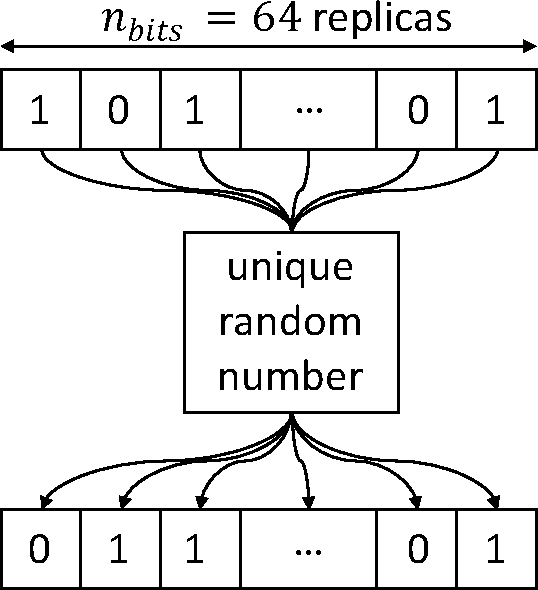
\includegraphics[height=5cm]{pictures/random_number.pdf}
\caption{All 64 replicas of a given spin share the same random number at each step.}
\label{fig:shared_rng}
\end{figure}

\subsection{Note on the independence of the realizations}
Because all replicas share the same sequence of random number, it is not obvious that their evolutions are independent. This is in fact guaranteed by two facts. The first one is that each replica is initialized independently of the others. The second one is that the shape of the energy landscape in each realization is also shaped independently of the others. Thus, the shared random number yields different outcome in each replica. A schematic view of this mechanism is shown in \Cref{fig:replica_independence}.

\begin{figure}[t]
\centering

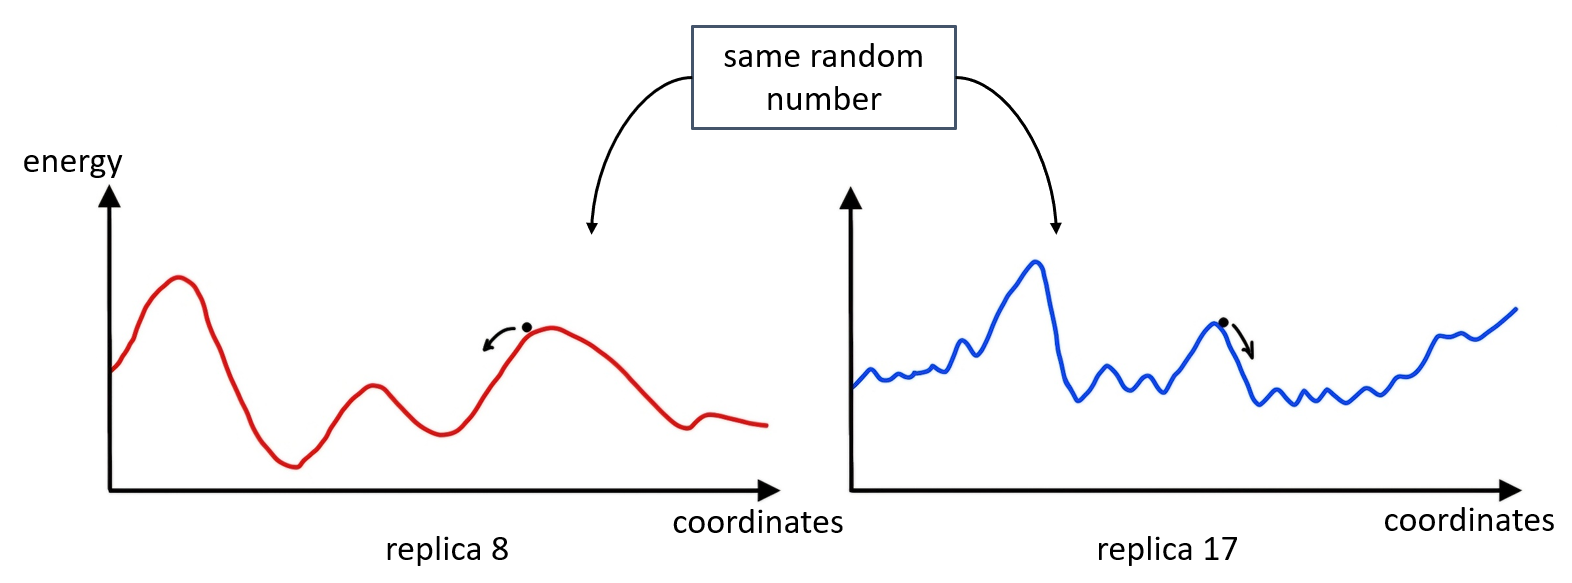
\includegraphics[width=\columnwidth]{replica_independence.png}
\caption{Schematic view of the independence of the realizations evolving from the same sequence of random numbers. Because of the unique energy landscape in every replica, and the independent initializations, the same random number yields independent evolutions.}
\label{fig:replica_independence}
\end{figure}

In a further analysis, one would be tempted to share the energy landscape across all replicas (this happens for instance if all replicas share the same patterns to be stored in the case of the Hopfield model, see subsection \ref{subsec:hopfield_model}). In this case, the realizations would be correlated through this shared energy landscape.

\subsection{Code structure}
We here present the structure of the code. It has been entirely written in \texttt{C++}, taking advantage of the object-oriented structure to factor out the common parts for each model while enabling them to evolve depending on their specificities. Most of the time of this internship has been spent understanding the object-oriented syntax and philosophy, and implementing an easily readable and efficient code for the simulation of the Metropolis algorithm on the different models. The structure found so far is presented in \Cref{fig:architecture}. Once the dynamics is simulated, the outputs are analyzed through python scripts.
\begin{figure}[t]
\centering

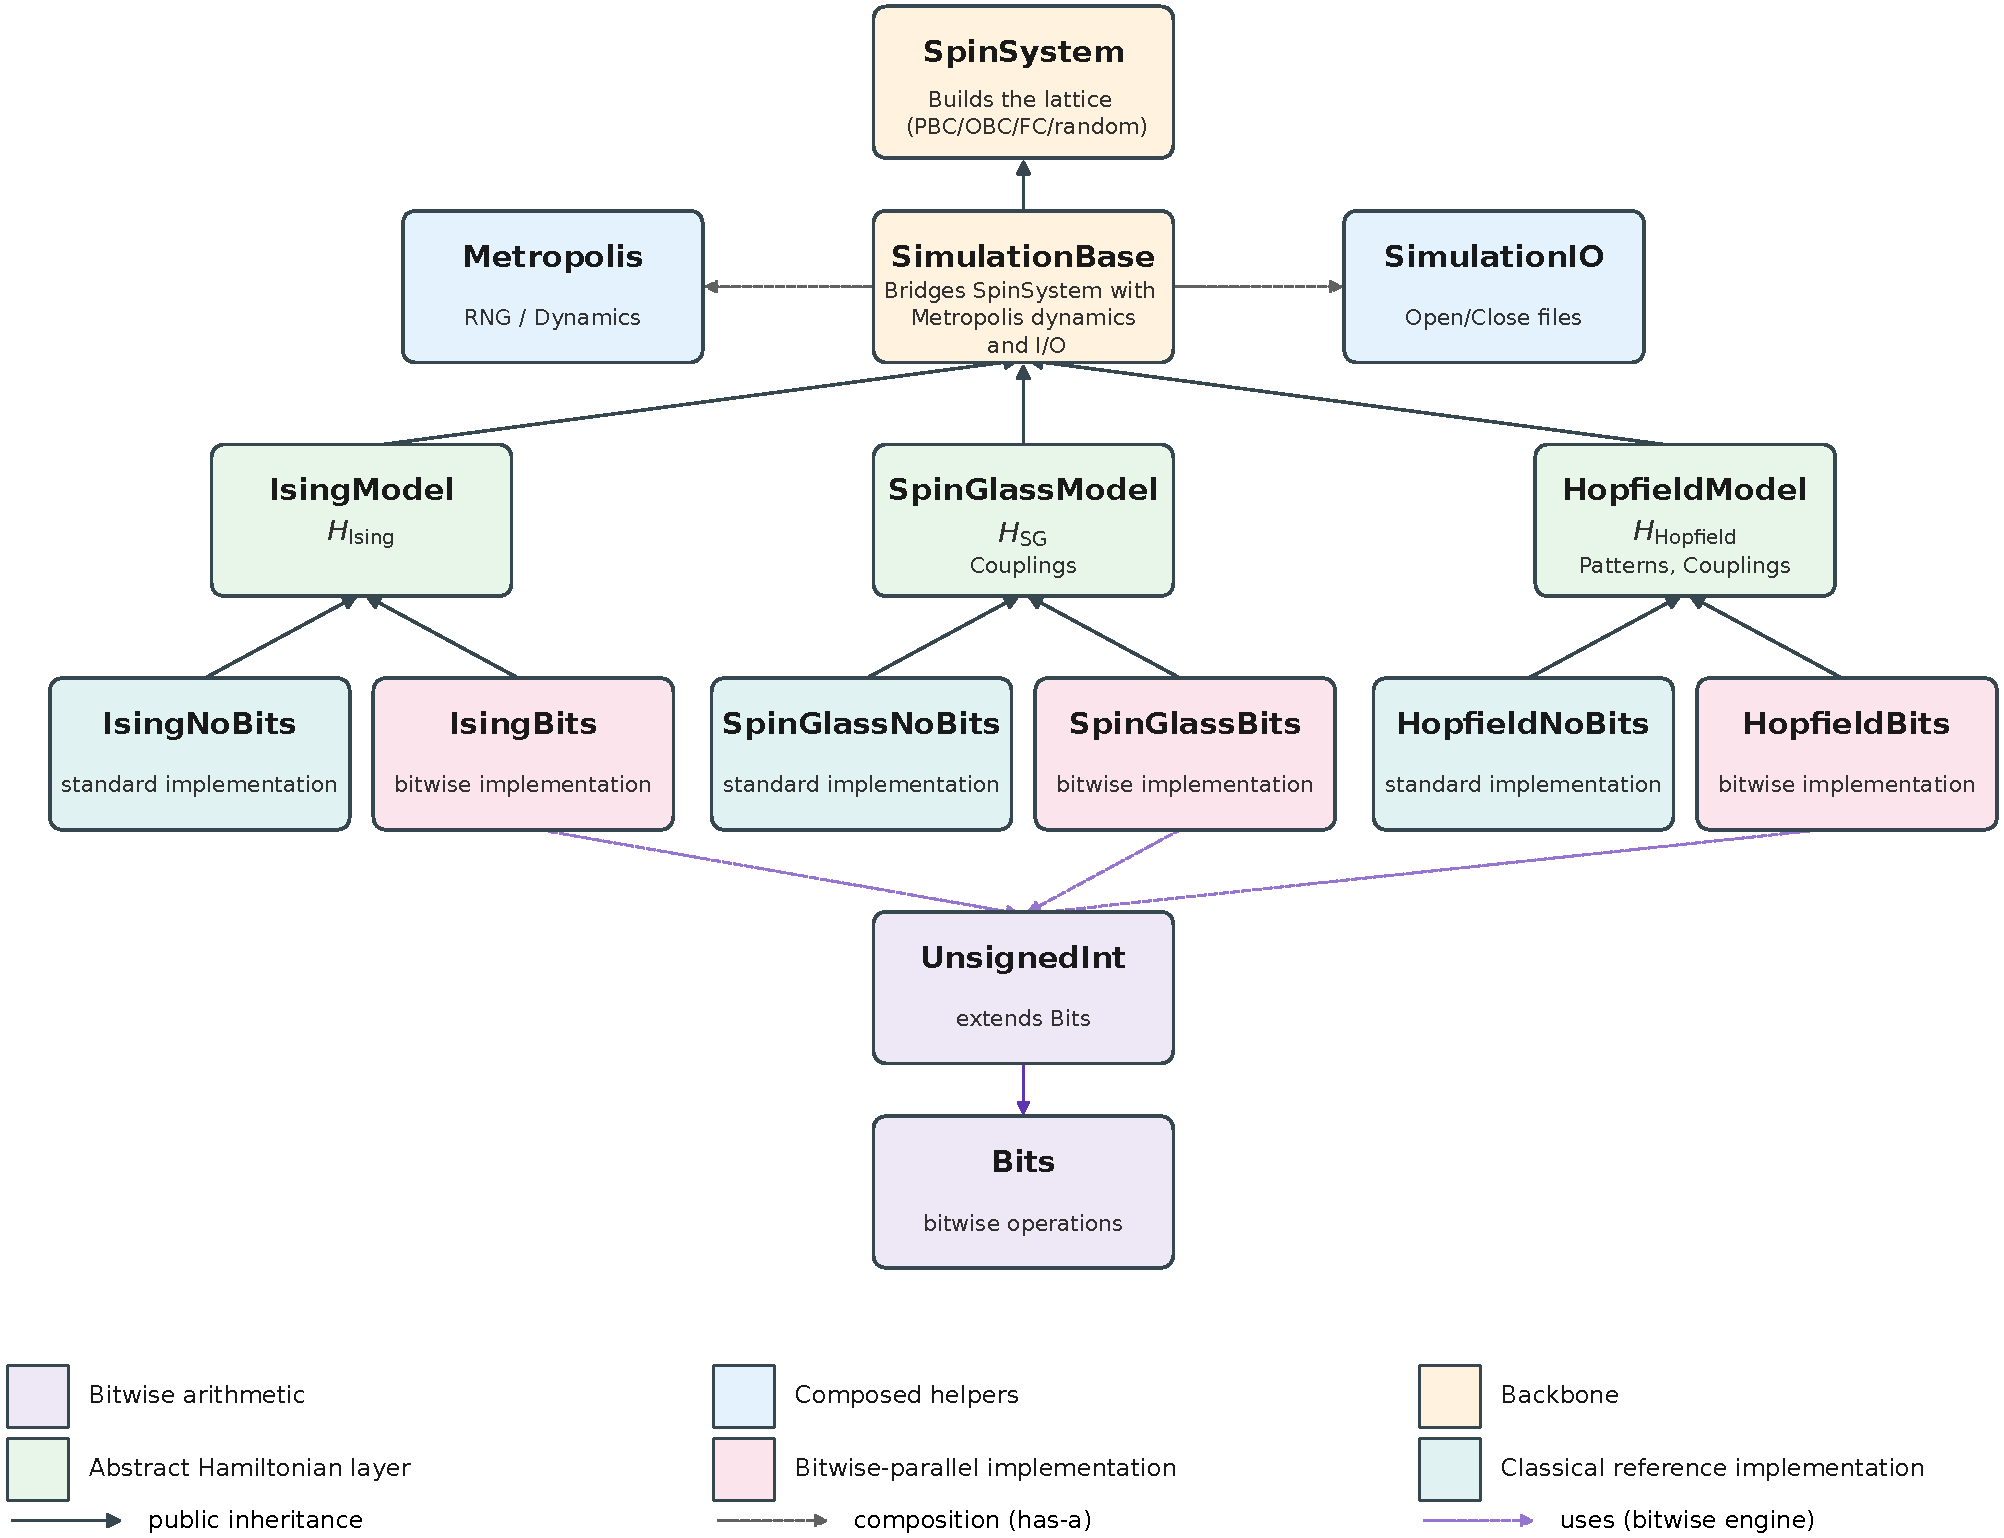
\includegraphics[width=\columnwidth]{architecture.pdf}
\caption{Code structure}
\label{fig:architecture}
\end{figure}
The code is built around hierarchical classes. We first implement the topology of the network, which is independent of the type of spin interaction and of the dynamical model considered. On this lattice, we set up the evolution rules (\textit{i.e.} the Metropolis algorithm in our case), and the input/output file management. Then, the combination (topology, dynamics) is applied to one of the three models implemented (Ising, Spin glass or Hopfield) and is implemented either in its standard or bitwise version. This code can be found in \cite{hopfield_code}.

\subsection{Standard implementation of the Metropolis algorithm}
We show here the standard implementation of the Metropolis algorithm, which will be broadly shared across all models.\\
If $\Delta E_k \leq 0$ the flip is accepted. Else, the flip condition $r \leq e^{-\beta \Delta E_k}$, yields:
\begin{equation}
\begin{aligned}
  \frac{-1}{\beta}\log r &\geq \Delta E_k\\
  \frac{-1}{\beta \kappa}\log r &\geq \Lambda_k,\\
\end{aligned}
\label{eq:flip_condition}
\end{equation}
with
\begin{equation}
  \Lambda_k \equiv \frac{\Delta E_k}{\kappa}.
  \label{eq:def_lambda}
\end{equation}
where  $\kappa$ corresponds to the constants of the model (\textit{i.e.} $2J$ in the case of the Hopfield model).
With $r \sim \mathcal{U}([0,1])$, we know that $-\log r \sim \mathcal{E}(1)$ , thus:
\begin{equation}
   \rho \equiv -\frac{1}{\beta \kappa}\log r  \sim \mathcal{E}(\beta \kappa).
\end{equation}
 The left-hand side of \Cref{eq:flip_condition} is a random variable of probability density $p(\rho)=\beta  \kappa e^{-\beta  \kappa \rho}$ and mean $(\beta  \kappa)^{-1}$.
The right-hand side of the equation is an integer which can be positive of negative. However, due to the first escape condition of the algorithm, we know that it is strictly positive. The left-hand side is thus compared with a positive integer. We can thus only consider the whole part of it without changing the inequality in order to obtain an integer-only flip condition:
\begin{equation}
  \lfloor \rho \rfloor \geq \Lambda_k,
  \label{eq:flip_int}
\end{equation}

A first naive implementation of the classical algorithm is given in the \Cref{alg:ising_classic_naive} in the appendix, where each of the $n_\text{bits}$ branch possesses its own random number. A more efficient implementation would be to share the drawn random threshold across the replicas. This shared random number version yields a fast escape condition, taking advantage of the inequality
\begin{equation*}
 -\max\Lambda_k \leq \Lambda_k \leq \max\Lambda_k ,
\end{equation*}
where $\max\Lambda_k $ only depend on the topology of the network.
Plugging this into Eq~\eqref{eq:flip_int} yields the flip escape condition:
\begin{equation}
 \lfloor \rho \rfloor \geq \max\Lambda_k
 \label{eq:flip_escape_condition}
\end{equation}
When satisfied, this guarantees that Eq.~\eqref{eq:flip_int} holds for every replica regardless of its local configuration, so that all replicas are flipped simultaneously without computing the per-replica test. This condition is typically met in the high-temperature regime, where $\rho$ is more likely to be large\\
We show in the \Cref{alg:ising_classic} the shared random number implementation of the Metropolis algorithm. This implementation is valid for all models, provided that the definition of $\kappa$ is adapted to each model.\\
\vspace{1em}
\begin{algorithm}[H]
\DontPrintSemicolon
\caption{Standard Metropolis implementation}
\KwIn{Lattice spins $\{S_i\}$, coupling $J$, inverse temperature $\beta$}
\KwOut{Updated lattice spins $\{S_i\}$}
\BlankLine
\BlankLine
\For{$\mathrm{sweep} = 1$ \KwTo $N_{\mathrm{sweeps}}$}{
    \For{$k = 1$ \KwTo $N$}{
      Draw $\lfloor \rho \rfloor$ with $\rho \sim \mathcal{E}(\beta \kappa)$\;
      \eIf{$\lfloor \rho \rfloor \geq \max\Lambda_k$}{
        \For{$r = 1$ \KwTo $n_\text{bits}$}{
            $s_k^{(r)} \leftarrow -s_k^{(r)}$\;
            }
        }{
            \For{$r = 1$ \KwTo $n_\text{bits}$}{
                Compute $\Lambda_k^{(r)} $\;
                \If{$\Lambda_k^{(r)} \leq 0$ \textbf{or} $\lfloor \rho \rfloor \geq \Lambda_k^{(r)}$}{
                    \BlankLine
                    \tcp{the test $\Lambda_k^{(r)} \leq 0$ is not necessary as $\lfloor \rho \rfloor$ has already been drawn, but is shown for pedagogy}
                    $s_k^{(r)} \leftarrow -s_k^{(r)}$\;
                }
            }
        }
    }
}
\label{alg:ising_classic}
\end{algorithm}
\vspace{1em}
This reduces the number of random draws per $n_\text{bits}$ cycle update to just one, shared among all replicas. This optimization is possible even though the structure is not fully parallelized across replicas. The only case for which this parallelized random number optimization might not be as efficient as expected is when $\Lambda_k^{(r)} \leq 0$  for all replicas simultaneously, in which case a random threshold is drawn but never used.
The complexity of this algorithm on a given network is $\mathcal{O}\left(N_\text{sweeps}\cdot N \cdot \langle n_\text{neighbor} \rangle \cdot n_\text{bits} \right)$.

\section{The Ising model}
We first implement the method on the Ising model, which is the simplest one.
\subsection{The model}
The Hamiltonian of the Ising network is given by
\begin{equation*}
  H_\text{Ising}=-J\sum_{\langle i,j \rangle}S_iS_j -h \sum_i S_i,
\end{equation*}
which, in absence of external field $h$ becomes,
\begin{equation}
  H_{\text{Ising, } h=0}=-J\sum_{\langle i,j \rangle}S_iS_j.
  \label{eq:ising}
\end{equation}
When flipping the spin $S_k$ ($S_k \to - S_k$), the associated energy shift is
\begin{equation}
\begin{aligned}
  \Delta E_k &= H_\text{Ising}\left[-S_k\right]-H_\text{Ising}\left[S_k\right] \\
  &= 2J S_k \sum_{i \in \partial k} S_i,
\end{aligned}
\label{eq:DeltaE_ising}
\end{equation}
where $i \in \partial k$ denotes the summation over the neighbors of $k$. Thus, here, $\kappa=2J$. We now need to implement the flip condition $m \geq \Lambda_k$ in a bitwise formalism in order to properly parallelize the evolutions.
\subsection{Bitwise Implementation}
Remembering that $S_i$ is actually an array containing $64$ replicas of the same spin, we write $S_i = -1 + 2B_i$, with $B_i$ a \Bits. The sum hence becomes:
\begin{equation*}
\begin{aligned}
  \sum_{i \in \partial k}S_k S_i&=\sum_{i \in \partial k} (-1+2B_k)(-1+2B_i)\\
                          &=\sum_{i \in \partial k} 1-2 (B_k+B_i) +4 B_k.B_i,\\
\end{aligned}
\end{equation*}
We show in Table~\ref{tab:XNOR} that the term in the sum can be re-written using the XNOR ($\odot$) logical operator.

\nolinenumbers
\begin{table}[h]
\centering
\begin{tabular}{cc||c|c|c}
\hline
$b_k$ & $b_i$ & $1- 2 (b_k+b_i) +4 b_k.b_i$ &  ${b_k \odot b_i}$ & $2{b_k \odot b_i} -1 $ \\
\hline
0 & 0 & $ \phantom{-}1$ & 1 & $\phantom{-}1$ \\
0 & 1 & $-1$ & 0  & $-1$ \\
1 & 0 & $-1$ & 0 &  $-1$ \\
1 & 1 & $\phantom{-}1$ & 1 & $\phantom{-}1$\\
\hline
\end{tabular}
\caption{The summed term can be simplified using a XNOR operator.}
\label{tab:XNOR}
\end{table}
\linenumbers

Thus, the term in the sum is simply equal to $2{B_k \odot B_i} -1 $, where $\odot$ denotes the bitwise XNOR operation applied to the corresponding bits of each \Bits. The sum can thus be written:
\begin{equation*}
  \sum_{i \in \partial k}S_k S_i=2\sum_{i \in \partial k} C_{ki} - n_k,
\end{equation*}
with $C_{ki}={B_k \odot B_i}$ and $n_k$ is the number of neighbor of the spin $k$. The bitwise flip condition is then:
\begin{equation}
 q+ n_k \geq 2 \sum_{i \in \partial k}C_{ki}.
  \label{eq:flip_ising_bitwise}
\end{equation}
 Moreover, the integer escape flip condition \eqref{eq:flip_escape_condition} (which translates in $m \geq n_k$) constrains the range of values taken by $q$ and $ 2 \sum_{i \in \partial k}C_{ki}$ to $n_k$ and $2n_k$, respectively (with $\max \Lambda_k = n_k$ in the case of the Ising network). This is particularly convenient, as it allows the \UnsignedInt objects to be allocated with static sizes at initialization, removing the need for dynamic resizing during the simulation.
 In addition, this integer flip condition can be applied to the bitwise algorithm and avoids the bitwise flipping test calculations for each replica: when it is met, all replicas are flipped simultaneously. A simple integer comparison suffices.\\

The pseudocode for the bitwise implementation of the Metropolis algorithm on this Ising network is presented in the \cref{alg:ising_bitwise}.\\
\nolinenumbers
\begin{algorithm}[b]
\DontPrintSemicolon
\caption{Bitwise Ising Metropolis}

\KwIn{Bit-replicated spins $\{B_i\}$, coupling $J$, inverse temperature $\beta$}
\KwOut{Updated lattice spins $\{S_i\}$}

\BlankLine
\textbf{Variables:} $\mathtt{Bits}\ \texttt{xnor},\ \texttt{mask}$\;
\phantom{\textbf{Variables:}} $\mathtt{UnsignedInt}\ T_k,\ \texttt{threshold}$\;

\For{$\mathrm{sweep}=1$ \KwTo $N_{\mathrm{sweep}}$}{
    \For{$\mathrm{step}=1$ \KwTo $N$}{
        Draw $k$ among $N$\;
        Draw $q$ with $\theta \sim \mathcal{E}(2\beta J)$

        \eIf{$m \ge n_k$}{
            $B_k \leftarrow \neg B_k$ \tcp*{escape condition: unconditional flip across all replicas}
        }{
            $T_k \leftarrow \mathbf{0}$

            $\mathtt{threshold} \leftarrow \mathbf{0}$

            \For{$i \in \partial k$}{
                $\mathtt{xnor}\ \leftarrow B_k \odot B_i$
                \tcp*{bitwise XNOR across replicas}

                $T_k \mathrel{+}= \mathtt{xnor}$
                \tcp*{increment agreement count per replica}
            }

            $T_k \leftarrow 2T_k$

            $\mathtt{threshold} \leftarrow q+n_k$

            $\mathtt{mask} \leftarrow (T_k \le \mathtt{threshold})$
            \tcp*{per-replica flip condition}

        $B_k \leftarrow B_k \oplus \mathtt{mask}$ \tcp*{bitwise spin flip (XOR operation): only replicas}
        \tcp*[r]{for which $\mathtt{mask}^{(\ell)}=1$ are flipped}
        }
    }
}

\label{alg:ising_bitwise}
\end{algorithm}
\linenumbers

\FloatBarrier
\subsection{Phase diagram}
We now need to make sure the bitwise implementation is consistent. This is firstly done by checking that it yields exactly the same spin configurations as the standard implementation with shared random numbers when starting from the exact same initial condition and using the same generative seed. Secondly, we can plot the phase diagram of the model and verify that it is in agreement with the known analytical results. We show in Figure~\ref{fig:phase_diagram_ising} the obtained phase diagram for several sizes of two-dimensional square lattices with periodic boundary conditions. This phase diagram is obtained by successive cooling the system: starting from the highest temperature, we progressively decrease it, using the final state of each step as the initial configuration for the next. This reduces the computational cost compared to reinitializing the network randomly at each temperature point, since the equilibrium state at each temperature lies close to that of the previous one, requiring fewer sweeps to reach thermalization. It aslo prevents the system to get stuck into metastable states such as the strip state for which several (usually two) regions of opposite magnetizations arise when the system is initialized randomly at a low temperature.\\

\nolinenumbers
\begin{figure}[htbp]
\centering

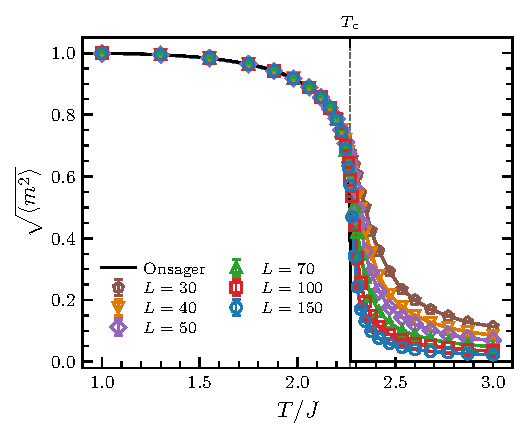
\includegraphics[width=\columnwidth]{pictures/magnetizations_multiN.pdf}
\caption{Phase diagram of the Ising model for several sizes of square lattices. The network is built with Periodic Boundary Conditions (PBC). The black line corresponds to the exact analytical solution found by Onsager in the case of an infinite square lattice \cite{Onsager1944}: $m(T)=0$ for $T\geq T_c$ and $m(T)_\pm= \pm \left[ 1 - \sinh^{-4}(2K) \right]^{1/8}$ for $T \leq T_c$, with $ K=J/T$ and $ T_c/J=2/\log\left(1+\sqrt 2\right)\approx 2.269$.}
\label{fig:phase_diagram_ising}
\end{figure}
\linenumbers

Qualitatively, it appears that the magnetization curves get closer to the exact solution when the lattice size is increased. This was to be expected as we gradually get closer to the infinite size case. We also notice an excellent agreement between the exact analytical magnetization and the obtained ones in the ferromagnetic part of the phase diagram. In this plot, each point corresponds to the mean over the $n_\text{bits}=64$ independent realizations. We show in Figure~\ref{fig:evolution_ising} the trajectories over time of the magnetizations for those 64 realizations at a given temperature.

\nolinenumbers
\begin{figure}[htbp]
\centering

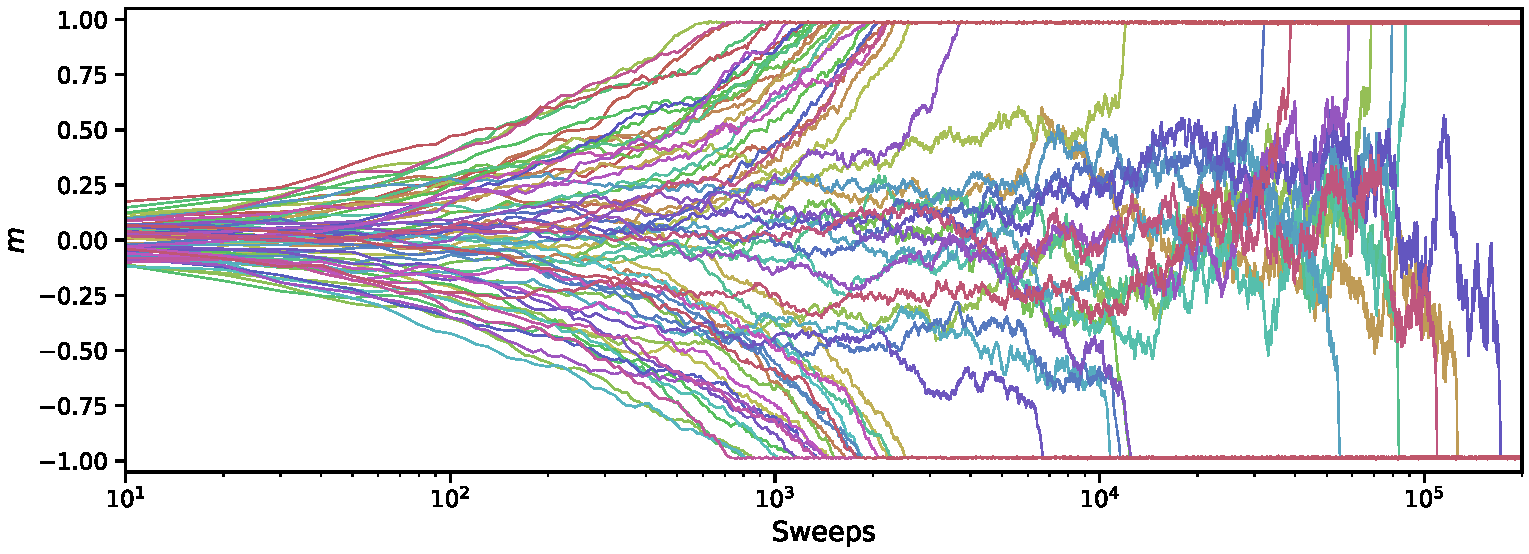
\includegraphics[width=\columnwidth]{pictures/evolution_ising_T1.5_L100.pdf}
\caption{Trajectories of the 64 magnetizations over time for $L=100$ and $T/J=1.5$. All those trajectories have been obtained from the same simulation. While some realizations quickly collapse into the equilibrium attractors $m_\pm = \pm 0.953$, some require $\sim 10^2$ times more sweeps to reach the same equilibrium.}
\label{fig:evolution_ising}
\end{figure}
\linenumbers

In order to make sure that the phase transition of the network indeed occurs at $T_c=2.269$ for all lattice sizes, we plot the Binder cumulant $U_L$, defined as:
\begin{equation}
  U_L = 1-\frac{\langle m^4 \rangle_L}{3\langle m^2 \rangle_L^2}
\end{equation}
Its limit values are $U_L(0)=2/3$ and $U_L(T \to \infty)=0$. Most importantly, it has been shown that all Binder curves for different lattice sizes $L$ intersect at the same scale-invariant critical point $\left(T_c,\, U^*\right)$ \cite{Binder1981}. This is because at $T_c$, the system becomes scale invariant, making the Binder cumulant independent of the system size at this specific temperature. We show in Figure~\ref{fig:binder} the plot of the Binder cumulants for the different lattice sizes. We obtain the expected curves, with the known asymptotic values and the crossing of the curves in $\left(T_c,\,U^*\right)$, which validates our implementation.

\nolinenumbers
\begin{figure}[htbp]
\centering
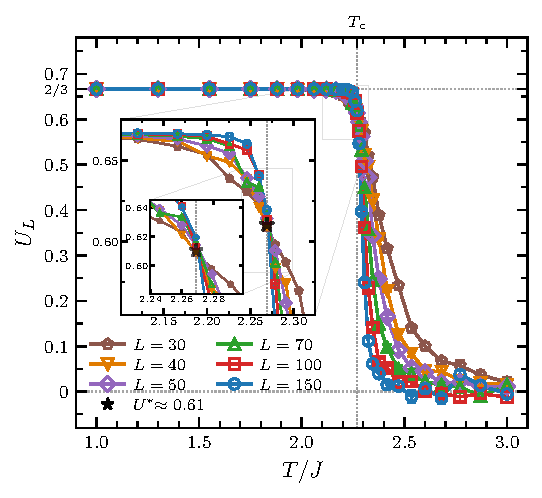
\includegraphics[width=\columnwidth]{binder_multiN.pdf}
\caption{Binder cumulant for the different lattice sizes. The curves approach the two asymptotic limits and intersect at $\left(T_c,\,U^*\right)$, as expected. Insets show the zoomed region around the critical point.}
\label{fig:binder}
\end{figure}
\linenumbers

\subsection{Performance test}
Now that our algorithm has been shown to produce correct results, we wish to estimate its performance compared to the usual naive implementation. To this end, we measure the ratio of the computational time required to let the system evolve over $2^{16}$ sweeps using both the classical naive and the bitwise implementation, for various square lattice sizes and temperatures. The result of this performance test is shown in \Cref{fig:speedup_ising}.

\nolinenumbers
\begin{figure*}[t]
\centering
% ── Top row ───────────────────────────────────────────────────────────────
\begin{minipage}[b]{0.49\textwidth}
\centering
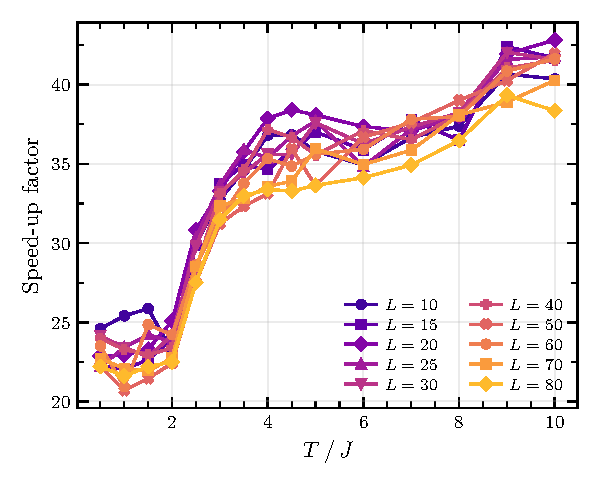
\includegraphics[width=\linewidth]{speedup_curves_ising.pdf}
\subcaption{Speedup factor evolution.}
\label{fig:speedup_curve_ising}
\end{minipage}
\hfill
\begin{minipage}[b]{0.49\textwidth}
\centering
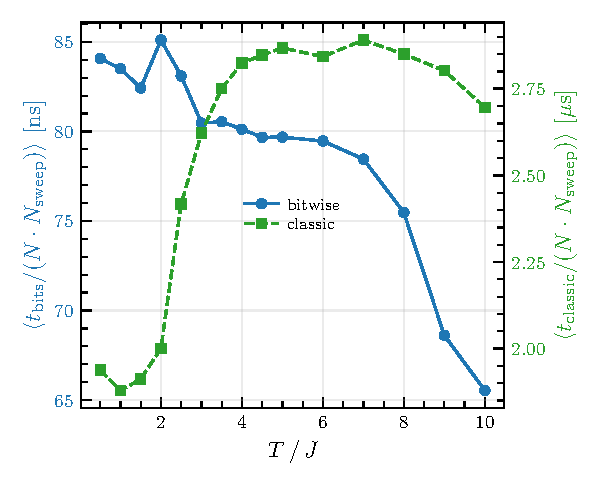
\includegraphics[width=\linewidth]{time_normalized_ising.pdf}
\subcaption{Normalized time evolution.}
\label{fig:normalised_time_ising}
\end{minipage}

\vspace{0.5em}

% ── Bottom row ────────────────────────────────────────────────────────────
\begin{minipage}[b]{\textwidth}
\centering
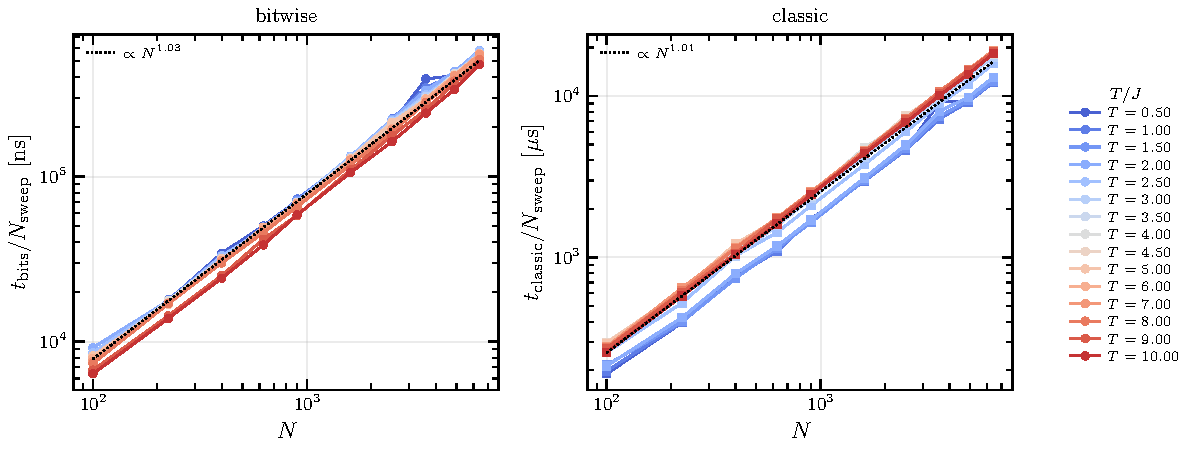
\includegraphics[width=\linewidth]{time_total_vs_N_ising.pdf}
\subcaption{Sweep time depending on the lattice size for all temperatures.}
\label{fig:sweep_time_vs_N_ising}
\end{minipage}

\caption{Performance analysis of the bitwise and classical Ising Metropolis implementations. Subfigure~(\subref{fig:speedup_curve_ising}) shows the evolution of the speedup factor with the temperature for several sizes of square lattices. (\subref{fig:normalised_time_ising}) shows the evolution of the normalized spin update time with the temperature, averaged over the different lattice sizes. Finally, (\subref{fig:sweep_time_vs_N_ising}) presents the evolution of the time taken to perform one sweep depending on the lattice size, for different temperatures.}
\label{fig:speedup_ising}
\end{figure*}
\linenumbers

The speedup factor lies between 20 and 45, which is a substantial performance increase. We notice that this speedup factor consistently increases with the temperature. As shown in (\subref{fig:sweep_time_vs_N_ising}), the early increase is mostly the effect of the ordering of the configurations at low temperature: before the phase transition, the state collapses into an ordered phase where all spins are aligned. This makes the unconditional flip condition $\Delta E_k \leq 0$ more frequent in the classical implementation, which is computationally cheaper, thus making it faster. This unconditional flip condition however becomes less probable when we increase the temperature, making the normalised time of the classic implementation and the speedup factor increase (especially near the critical temperature $T_c$) up to a certain value where the normalised time stops increasing, probably as the unconditional flip condition is never met anymore. We also notice that the unconditional flip condition in the bitwise implementation ($m \geq n_k$) becomes more and more probable with the increasing temperature, making the bitwise implementation faster. These two effects combined explain the overall shape of the speedup factor evolution, where the first increase is coming from the classical implementation and the second one is the effect of the bitwise. It should be noted that this overall tendency may not be observed in the case of a comparison with the standard Metropolis algorithm, as the non-naive standard Metropolis implementation possesses the same escape condition $m \geq n_k$, making it faster and thus slowing down (or supressing) the second increase in the speedup factor. \\
The increase seems to be uncorrelated with the size of the system. In theory, the speedup factor can even be larger than 64, as the structural optimization alone can potentially yield a speedup of 64 by itself, as it enables us to make 64 realizations evolve in parallel. However, this structural optimization comes with the cost of creating and storing the bitwise objects used to parallelize the evolution, thus reducing the net performance improvement.\\
The Subfigure~(\subref{fig:sweep_time_vs_N_ising}) shows that the time required grows proportionally to the system size for both implementation. The complexity of the bitwise implementation thus seems to be $\mathcal{O}\left(N_\text{sweeps} \cdot  N \cdot \langle n_\text{neighbor} \rangle \right)$.
It must be noted that, while we here measure an increase in the speed of the code for a fixed number of outputs, the true advantage of the bitwise implementation is to produce more independent results within the same computational time.

\section{The Spinglass model}
We now move on a more complex model, in order to approach the structure of the Hopfield network.
\subsection{The Edwards–Anderson model}
The Edwards–Anderson (EA) model -- first introduced by Edwards and Anderson in 1975 \cite{SFEdwards_1975} -- is a finite dimensional spin glass model with short range interaction. It is not a mean field spin glass model with infinite range interactions such as the Sherrington–Kirkpatrick model \cite{SK_model}. The model is formally described as follows:
\begin{equation}
  H_\text{EA}=\sum_{\langle i,j \rangle}J_{ij}S_iS_j.
  \label{eq:EA_model}
\end{equation}
Where $J_{ij}$ is a random variable taking its values in $\{-1,\,1\}$ with equal probability. Thus, it can easily be represented by a \Bits.
Under a spin flip ($S_k \to - S_k$), the energy shift is:
\begin{equation}
  \Delta E_k=2 S_k \sum_{i \in \partial k}J_{ki}S_i.
  \label{eq:DeltaE_EA}
\end{equation}
The structure being really similar to that of \eqref{eq:DeltaE_ising}, we can perform the same derivation as for the Ising model and find the spin flip condition:
\begin{equation}
  \lfloor \rho \rfloor \geq S_k  \sum_{i \in \partial k}J_{ki}S_i,\\
  \label{eq:flip_EA_int}
\end{equation}
with this time $\rho \sim \mathcal{E}(2\beta)$.
\subsection{Bitwise Implementation}
We now need to express the product $J_{ik}S_kS_i$ in a binary way. As shown in the previous section, the product $S_kS_i$ can be re-written $(-1+2B_k)(-1+2B_i)=-1+2 C_{ki}$ with $C_{ki}= B_k \odot B_i$. Thus, by writing $J_{ki}=-1+2K_{ki}$ with $K_{ki}$ a \Bits, we have:
\begin{equation*}
  \begin{aligned}
  J_{ik}S_kS_i =& (-1+2K_{ki})(-1+2 C_{ki})\\
               =& -1 + 2D_{ki},\\
  \end{aligned}
\end{equation*}
with $D_{ki}=K_{ki}\odot C_{ki}= K_{ki} \odot B_k \odot B_i =  K_{ki} \oplus B_k \oplus B_i$. As in the previous section, the flip condition is then:
\begin{equation}
  \lfloor \rho \rfloor + n_k \geq 2 \sum_{i \in \partial k}D_{ki}.
  \label{eq:flip_SG_bitwise}
\end{equation}
Both the bitwise and the classic implementation are thus similar to this of the Ising model, and we will not present them further in this report. The bitwise algorithm for the spin glass model can be found in the appendix, see \Cref{alg:SG_bitwise}.\\
The bitwise implementation is not validated here, as the bitwise framework was already tested in the previous section, and the main interest of this model lies in bridging the complexity gap between the Ising model and the Hopfield network. We nonetheless verified that the standard and the bitwise implementations produce identical spin configurations when initialized from the same initial state and driven by the same sequence of random numbers.
\begin{algorithm}[t]
\DontPrintSemicolon
\caption{Bitwise spin glass Metropolis}

\KwIn{Bit-replicated spins $\{B_i\}$, couplings $\texttt{Couplings}$, neighbor lists $\partial i$, inverse temperature $\beta$}
\KwOut{Updated spin configurations $\{B_i\}$}

\BlankLine
\textbf{Preallocated variables:} $\mathtt{Bits}\ \texttt{xnor},\ \texttt{mask}$\;
\phantom{\textbf{Preallocated variables:}} $\mathtt{UnsignedInt}\ T_i,\ \texttt{threshold}$\;

\BlankLine

\For{$\mathrm{sweep}=1$ \KwTo $N_{\mathrm{sweeps}}$}{
    \For{$\mathrm{step}=1$ \KwTo $N$}{
        Draw $k$ among $N$\;
        Draw $\lfloor \rho \rfloor$ with $\rho \sim \mathcal{E}(2\beta)$

        \eIf{$\lfloor \rho \rfloor \ge n_k$}{
            $B_k \leftarrow \neg B_k$ \tcp*{escape condition: unconditional flip across all replicas}
        }{
            $T_k \leftarrow \mathbf{0}$

            $\mathtt{threshold} \leftarrow \mathbf{0}$

            \For{$i \in \partial k$}{
                $\mathtt{xnor}\ \leftarrow K_{ki} \oplus B_k \oplus B_i$
                \tcp*{bitwise XNOR across replicas}

                $T_k \mathrel{+}= \mathtt{xnor}$
                \tcp*{increment agreement count per replica}
            }

            $T_k \leftarrow 2T_k$

            $\mathtt{threshold} \leftarrow \lfloor \rho \rfloor +n_k$

            $\mathtt{mask} \leftarrow (T_k \le \mathtt{threshold})$
            \tcp*{per-replica flip condition}

        $B_k \leftarrow B_k \oplus \mathtt{mask}$ \tcp*{bitwise spin flip (XOR operation): only replicas}
        \tcp*[r]{for which $\mathtt{mask}^{(\ell)}=1$ are flipped}
        }
    }
}

\label{alg:SG_bitwise}
\end{algorithm}
\FloatBarrier
\subsection{Performance test}
 We now test the performance of the implementation, for several lattice sizes and the temperatures, this time with $N_\text{sweeps}=2^{14}$. The results are shown in \Cref{fig:speedup_spinglass}. We notice the same evolution of the normalized time for both implementation as the ones observed for the Ising model. The shape of the speedup factor is similar to this of the Ising model, but its evolution is steadier, with what appears to be a saturation for the highest temperatures. The time per sweep also remains proportional to the system size, the complexities of the implementations thus should be similar to those of the Ising model.

\clearpage
\newpage
\FloatBarrier


\nolinenumbers
\begin{figure}[htbp]
\centering
% ── Top row ───────────────────────────────────────────────────────────────
\begin{minipage}[b]{0.49\textwidth}
    \centering
    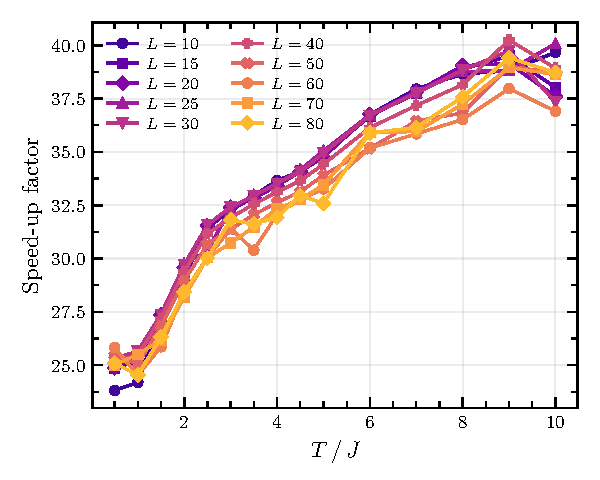
\includegraphics[width=\columnwidth]{speedup_curves_spinglass.pdf}
    \subcaption{Speedup factor evolution.}
    \label{fig:speedup_curve_spinglass}
\end{minipage}
\hfill
\begin{minipage}[b]{0.49\textwidth}
    \centering
    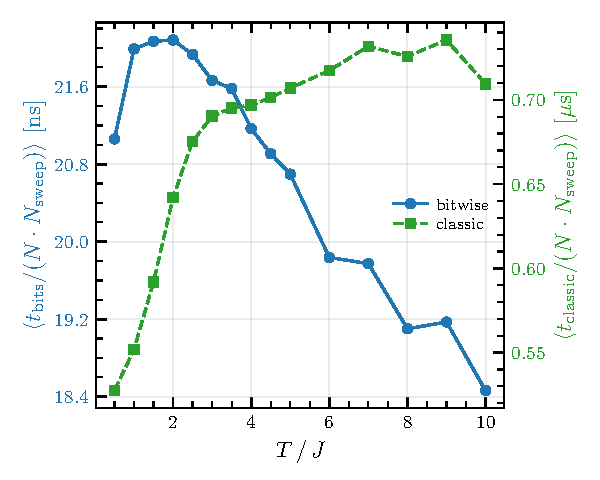
\includegraphics[width=\columnwidth]{time_normalized_spinglass.pdf}
    \subcaption{Normalized time evolution.}
    \label{fig:normalised_time_spinglass}
\end{minipage}

\vspace{0.5em}

% ── Bottom row ────────────────────────────────────────────────────────────
\begin{minipage}[b]{\textwidth}
    \centering
    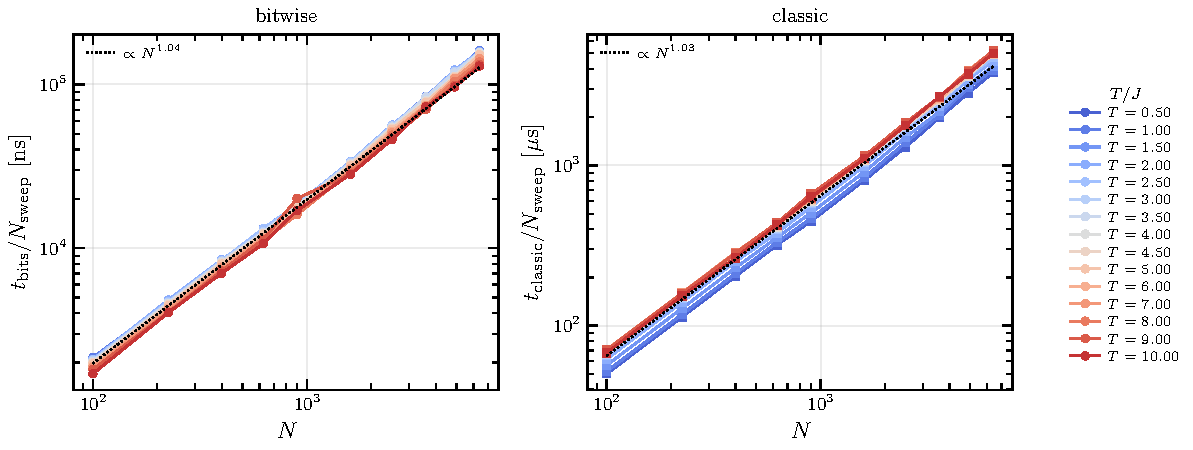
\includegraphics[width=\columnwidth]{time_total_vs_N_spinglass.pdf}
    \subcaption{Sweep time depending on the lattice size for all temperatures.}
    \label{fig:sweep_time_vs_N_spinglass}
\end{minipage}
\caption{Performance analysis of the bitwise and classical Spin Glass Metropolis implementations.}
\label{fig:speedup_spinglass}
\end{figure}
\linenumbers
\FloatBarrier

\section{The Hopfield model}
We here present the Hopfield model, which is of interest in this internship.
\subsection{The model}
\label{subsec:hopfield_model}
The Hopfield Hamiltonian resemble this of the spin glass model and is as follows:
\begin{equation}
  H_\text{Hopfield}=-\frac{1}{2}\sum_{i \neq j}w_{ij}S_iS_j,
  \label{eq:Hopfield}
\end{equation}
where in this case the weights $w_{ij}$ are not initialized randomly but rather determined by a set of states that one wants to ``store'' in the network (this term will be explained further on):
\begin{equation}
  w_{ij}=\frac{1}{N}\sum_{\mu=1}^{p} \xi_i^\mu \xi_j^\mu.
\end{equation}
With $\{\xi^1, \xi^2 \ldots, \xi^p\}$ the set of patterns to be memorized by the network, each pattern being a state of the system with components $\xi_i^\mu = \pm 1$. This initialization follows the Hebb rule ``neurons that fire together wire together'' \cite{Hebb1949}. By setting the weights this way, the energy landscape is shaped with local minima at each pattern coordinates.

By initializing the network not far from one of the stored patters, the dynamics will make it tend to the precise pattern's configuration, given that we are located in the memory phase of the model. In this way, the network is said to have associative memory: it can recover a stored pattern from a partial or noisy version of that pattern. A visual representation of the model is shown in \Cref{fig:energy_landscape}.

A parameter of particular interest in this model is its storage load, defined as the number of patterns to be stored over the size of the network: $\alpha = p /N$ with p the number of patterns to be stored. The equilibrium properties of the model, depending both on the temperature and on this storage load have been extensively studies in \cite{Amit1985,AMIT1987,Amit1989,Sompolinsky1988}. We show in \Cref{fig:phase_diagram_hopfield} the phase diagram of the Hopfield model on a fully-connected network, which is the reference topology of the model. In the limit $T\to0$, the model is known to exhibit a phase transition at $\alpha_c= 0.138$. This critical storage load value can be regarded as the network’s storage capacity, as beyond this threshold the model is no longer able to reconstruct the stored data from partial or corrupted data. Above the network's capacity, the energy minima overlap, leading to mixed or spurious (parasite) states that prevent accurate retrieval of stored information.

In order to study the capacity of the network to recover stored data, we introduce the overlap order parameter:
\begin{equation}
    m^\mu = \frac{1}{N}\sum_{i=1}^N \xi_i^\mu S_i.
\end{equation}
This quantity measures how much the system's configuration is aligned with the pattern $\mu$.
Using the definition of $m^\mu$, the energy of the system can be re-written:
\begin{equation}
  E=-\frac{N}{2}\sum_{\mu=1}^{p} (m^\mu)^2.
\end{equation}

All the $m^\mu$ are of order $1/\sqrt{N}$ for a state that is uncorrelated with the memories, while, in the memory phase, $m^*$ should be of the order of the unit \cite{Sompolinsky1988}. Thus, we often consider the pattern for which the overlap is maximum: $m^* = \max\limits_\mu |m^\mu|$. We take the absolute value of the overlap as the system can also end up in the configuration opposite of the stored pattern due to the $\mathbb{Z}_2$ global spin flip symmetry.  From $m^*$ we can define the reconstruction error of the network:
\begin{equation}
    \text{error}=\frac{1-m^*}{2}
\end{equation}

We show in \Cref{fig:phase_transition} the evolution of the error with the storage load:
\nolinenumbers
\begin{figure}[t]
\centering
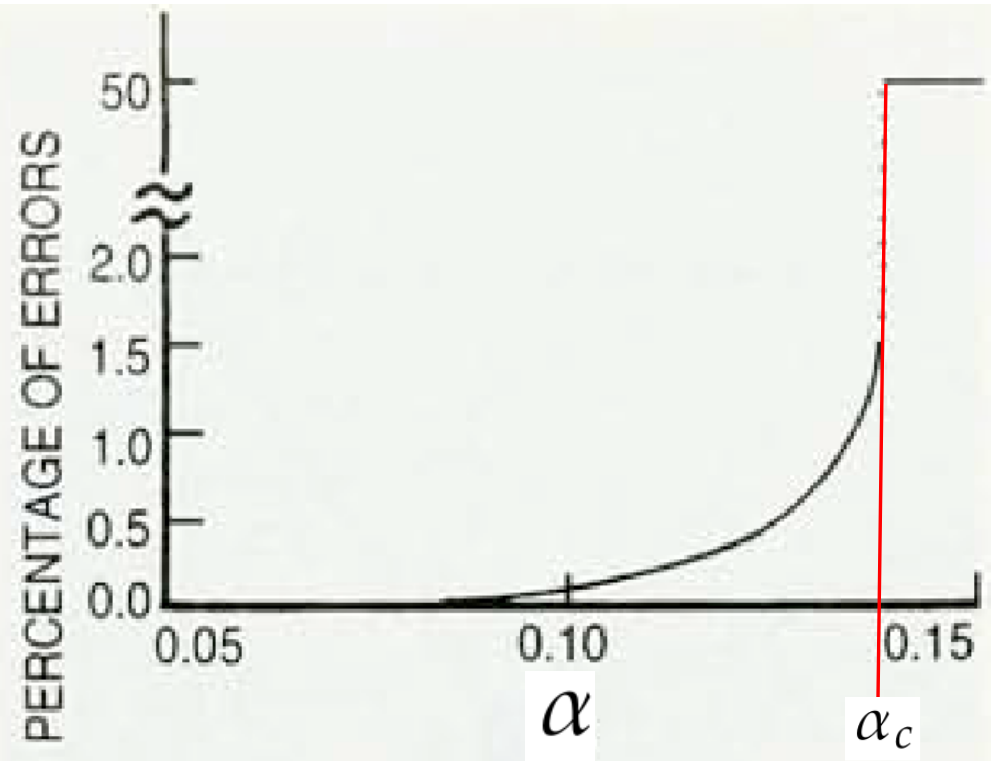
\includegraphics[width=0.6\columnwidth]{phase_transition.png}
\caption{Evolution of the error with the storage load, extracted from \cite{Sompolinsky1988}.  For this diagram, the configuration is initialized near a pattern. When the storage load exceeds $\alpha_c$, the configuration becomes totally uncorrelated with the stored patterns and the error suddenly jumps to 0.5.}
\label{fig:phase_transition}
\end{figure}
\linenumbers
\include{Conclusion}
\begin{appendix}
\section*{Appendices}
\addcontentsline{toc}{section}{Appendices}

% Pour s'assurer que seules les sous-sections apparaissent dans la TOC
\addtocontents{toc}{\protect\setcounter{tocdepth}{2}}

% Redéfinition de la numérotation des sous-sections pour les appendices
\renewcommand{\thesubsection}{\Alph{subsection}}

% Appendix A

\linenumbers
\subsection{Bitwise implementation of the Metropolis algorithm for the spin glass model}
\nolinenumbers

\linenumbers
\FloatBarrier
\end{appendix}

\setlength{\bibsep}{2pt}
\bibliographystyle{unsrt}
\bibliography{references}

\end{document}
